% Gauss, Werke X/1 (1917), native67–68, printed60–61.
\SourceLeaf{067}\ArithmeticHead{60}{L}{ARITHMETIK.\quad NACHLASS.}
\par\indent[7.] Ferner wird
\[
\begin{aligned}
m&=\tfrac18(D-1)+\tfrac14b-\nu\\
n&=\tfrac18(D-1)-\tfrac14b+\nu.
\end{aligned}
\]
\noindent Also der Decident von $1+i$
\[
\begin{aligned}
{}&=\tfrac58(D-1)+\tfrac14b-\nu\\
&=\tfrac58(D-1)+\tfrac14ab+h,
\end{aligned}
\]
\noindent wo
\[
\begin{array}{rclllll}
h={}&0&\text{für}&a&\text{[von der]}&\text{Form}&8n+1,8n+7,\\
&2&\text{„}&\text{„}&\text{„\quad „}&\text{„}&8n+3,8n+5;
\end{array}
\]
\noindent man kann dafür auch $\dfrac{aa-1}{4}$ setzen.
\[
\begin{aligned}
\tfrac18\{5aa+5bb-5+2ab+2aa-2\}&=\tfrac18(7aa+2ab+5bb-7)\\
&\equiv\tfrac18(-aa+2ab-3bb+1),
\end{aligned}
\]
\noindent da die Differenz
\[
{}=aa+bb-1.
\]
\noindent So ist das Theorem, die obige Induction als richtig angenommen, bewiesen.
\begin{center}\textit{Grösseres Tableau der $m,n$,}\end{center}
\begingroup\small\setlength{\tabcolsep}{5pt}\renewcommand{\arraystretch}{1.12}
\begin{center}
\begin{tabular}{r|r||r|r||r|r||}
$1+2i$&1.0&$3+2i$&1.2&$5+2i$&4.3\\
$1+4i$&3.1&$3+4i$&4.2&$5+4i$&4.6\\
$1+6i$&6.3&$3+6i$&6.5&$5+6i$&9.6\\
$1+8i$&10.6&$3+8i$&9.9&$5+8i$&11.11\\
$1+10i$&13.10&$3+10i$&15.12&$5+10i$&16.15\\
$1+12i$&21.15&$3+12i$&19.17&$5+12i$&22.20\\
$1+14i$&28.21&$3+14i$&26.25&$5+14i$&27.28\\
$1+16i$&36.28&$3+16i$&35.31&$5+16i$&37.33\\
$1+18i$&45.36&$3+18i$&43.40&$5+18i$&44.43\\
$1+20i$&55.45&$3+20i$&52.50&$5+20i$&54.52\\
$1+22i$&66.55&$3+22i$&64.59&$5+22i$&65.62
\end{tabular}
\par\medskip
\begin{tabular}{r|r||r|r||r|r}
$7+2i$&6.7&$9+2i$&11.10&$11+2i$&15.16\\
$7+4i$&7.9&$9+4i$&13.11&$11+4i$&18.16\\
$7+6i$&9.12&$9+6i$&14.15&$11+6i$&18.21\\
$7+8i$&16.12&$9+8i$&16.20&$11+8i$&23.23\\
$7+10i$&20.17&$9+10i$&25.20&$11+10i$&25.30\\
$7+12i$&25.23&$9+12i$&29.27&$11+12i$&36.30\\
$7+14i$&31.30&$9+14i$&34.35&$11+14i$&40.39\\
$7+16i$&38.38&$9+16i$&42.42&$11+16i$&49.45\\
$7+18i$&46.47&$9+18i$&51.50&$11+18i$&55.56\\
$7+20i$&55.57&$9+20i$&61.59&$11+20i$&66.64\\
$7+22i$&69.64&$9+22i$&72.69&$11+22i$&76.75
\end{tabular}
\end{center}\endgroup
\par\indent Eine besondere Untersuchung verdient die Anzahl der geraden und ungeraden [Zahlen] im ersten Quadranten. Sie ist respective der Zahl aller in $A$ und $B$ gleich.
\clearpage

\SourceLeaf{068}\ArithmeticHead{61}{R}{ZUR THEORIE DES BIQUADRATISCHEN RESTES $1+i$.}
\begin{center}
\begin{tikzpicture}[x=.75cm,y=.75cm,line width=.4pt]
\draw (0,0)--(0,2)--(2,2)--(2,0)--cycle;
\draw (0,0)--(2,2);
\node at (.57,1.46) {$B$};\node at (1.46,.55) {$A$};
\node[anchor=east,inner sep=1pt] at (0,0) {$\tfrac12m$};
\node[anchor=west,inner sep=1pt] at (2,0) {$0$};
\node[anchor=west,inner sep=1pt] at (2,2) {$\tfrac12mi$};
\end{tikzpicture}
\par\smallskip Das Zeichen von $i$ ändert nichts.
\end{center}
\begingroup\small\setlength{\tabcolsep}{5pt}\renewcommand{\arraystretch}{1.12}
\begin{center}
\begin{tabular}{r|r@{\qquad}r|r@{\qquad}r|r}
$1+2i$&0.1&$5+6i$&6.9&$1+10i$&12.13\\
$3+2i$&2.1&$1+8i$&8.8&$3+10i$&14.13\\
$1+4i$&2.2&$7+4i$&8.8&$7+8i$&12.16\\
$3+4i$&2.4&$3+8i$&8.10&$11+2i$&16.15\\
$5+2i$&4.3&$9+2i$&10.11&$11+4i$&18.16\\
$1+6i$&4.5&$7+6i$&12.9&$1+12i$&18.18\\
$5+4i$&6.4&$5+8i$&10.12&$9+8i$&20.16\\
$7+2i$&6.7&$9+4i$&12.12&$7+10i$&18.19
\end{tabular}
\par\medskip
\begin{tabular}{r|r@{\qquad}r|r}
$11+6i$&20.19&$3+14i$&26.25\\
$5+12i$&20.22&$13+6i$&25.25\\
$13+2i$&22.21&\multicolumn{1}{r}{}&\\
$9+10i$&20.25&\multicolumn{1}{r}{}&\\
$11+8i$&24.22&\multicolumn{1}{r}{}&\\
$13+4i$&22.24&\multicolumn{1}{r}{}&\\
$7+12i$&24.24&\multicolumn{1}{r}{}&\\
$1+14i$&24.25&\multicolumn{1}{r}{}&
\end{tabular}
\end{center}\endgroup
\noindent Dass die Zahlen der ersten Colonne immer gerade sind, beweiset man daher, dass, wenn die Summe aller Zahlen im ersten Quadr. $=t+iu$ ist, und
\[
(a-bi)(t+iu)=T+iU
\]
\noindent gesetzt wird, man
\[
T+U=\tfrac18(pp-1)
\]
\noindent hat etc.
\NumberedItem{2}
\par\indent Das obige nur auf Induction gegründete Lemma wird durch folgendes ersetzt.

Man hat für $a,b-a$ positiv
\[
M=-P+Q-R
\]
\noindent wo
\[
\begin{aligned}
P&=\left[\frac ba\right]+\left[\frac{2b}a\right]+\left[\frac{3b}a\right]+\ldots+\left[\frac{\tfrac12(a-1)b}a\right]\\
&=\varphi(a,b)=\tfrac14(a-1)b-\varphi(b,a)
\end{aligned}
\]
\[
\begin{aligned}
Q&=\left[\tfrac12b+\frac a{2b}\right]+\left[\tfrac12b+\frac{3a}{2b}\right]+\left[\tfrac12b+\frac{5a}{2b}\right]+\ldots+\left[\tfrac12b+\frac{(b-1)a}{2b}\right]\\
&=\tfrac14bb+\varphi(2b,a)-\varphi(b,a)
\end{aligned}
\]
\[
\begin{aligned}
R&=\left[\frac{b+a}{b-a}\right]+\left[\frac{2(b+a)}{b-a}\right]+\left[\frac{3(b+a)}{b-a}\right]+\ldots+\left[\frac{\tfrac12(b-a-1)(b+a)}{b-a}\right]\\
&=\varphi(b-a,b+a).
\end{aligned}
\]
\clearpage
